\documentclass[tikz,border=5pt]{standalone}
\usepackage{xcolor}

\begin{document}
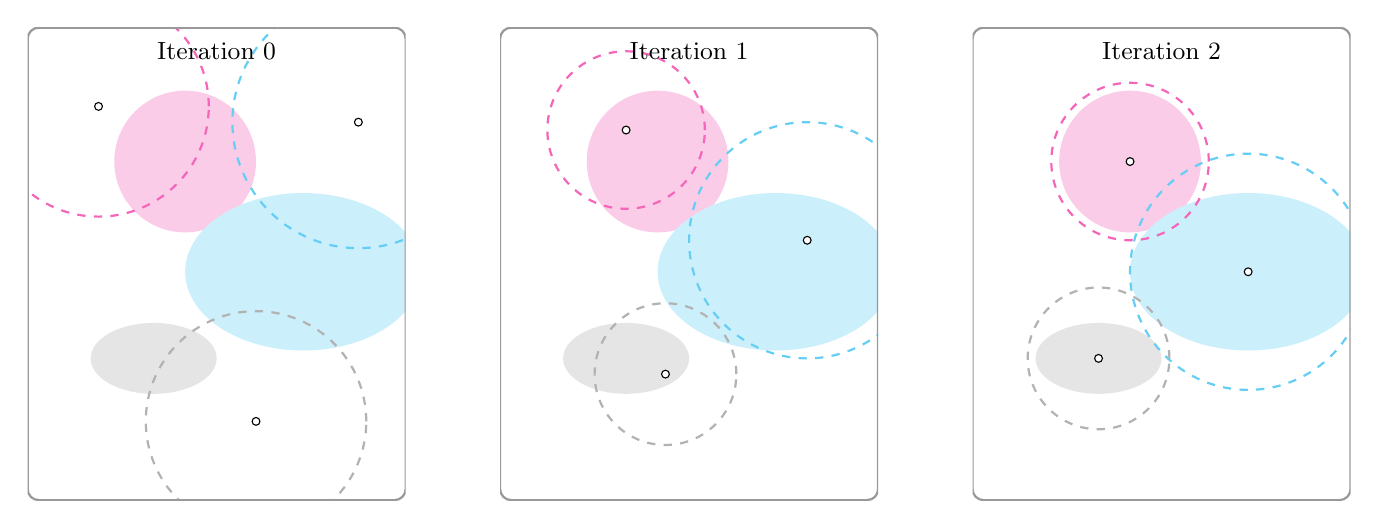
\begin{tikzpicture}[scale=1]

% ---------- common style ----------
\tikzstyle{panel}=[draw=black!40,rounded corners,thick]
\tikzstyle{center}=[circle,draw=black,fill=white,inner sep=1pt]

% ================== Panel 1: initial assignment ==================
\begin{scope}[shift={(0,0)}]
  % clip region
  \clip (-2.4,-3) rectangle (2.4,3);

  % data blobs (new color scheme)
  \fill[magenta!20] (-0.4,1.3) circle (0.9);               % magenta blob
  \fill[gray!20]   (-0.8,-1.2) ellipse (0.8 and 0.45);     % gray blob
  \fill[cyan!20]   (1.1,-0.1)  ellipse (1.5 and 1.0);      % cyan blob

  % initial (bad) centers
  \node[center] (c1a) at (-1.5,  2.0) {};
  \node[center] (c2a) at ( 1.8,  1.8) {};
  \node[center] (c3a) at ( 0.5, -2.0) {};

  % dashed circular decision regions
  \draw[magenta!60,dashed,thick] (c1a) circle (1.4);
  \draw[cyan!60,dashed,thick]    (c2a) circle (1.6);
  \draw[gray!60,dashed,thick]    (c3a) circle (1.4);

  % frame + title (also inside clip)
  \draw[panel] (-2.4,-3) rectangle (2.4,3);
  \node at (0,2.7) {\small Iteration 0};
\end{scope}

% ================== Panel 2: updated centers ==================
\begin{scope}[shift={(6,0)}]
  \clip (-2.4,-3) rectangle (2.4,3);

  % same data blobs
  \fill[magenta!20] (-0.4,1.3) circle (0.9);
  \fill[gray!20]   (-0.8,-1.2) ellipse (0.8 and 0.45);
  \fill[cyan!20]   (1.1,-0.1)  ellipse (1.5 and 1.0);

  % means after one update
  \node[center] (c1b) at (-0.8, 1.7) {};
  \node[center] (c2b) at ( 1.5,0.3) {};
  \node[center] (c3b) at (-0.3,-1.4) {};

  % dashed regions
  \draw[magenta!60,dashed,thick] (c1b) circle (1.0);
  \draw[cyan!60,dashed,thick]    (c2b) circle (1.5);
  \draw[gray!60,dashed,thick]    (c3b) circle (0.9);

  \draw[panel] (-2.4,-3) rectangle (2.4,3);
  \node at (0,2.7) {\small Iteration 1};
\end{scope}

% ================== Panel 3: converged ==================
\begin{scope}[shift={(12,0)}]
  \clip (-2.4,-3) rectangle (2.4,3);

  % same data blobs
  \fill[magenta!20] (-0.4,1.3) circle (0.9);
  \fill[gray!20]   (-0.8,-1.2) ellipse (0.8 and 0.45);
  \fill[cyan!20]   (1.1,-0.1)  ellipse (1.5 and 1.0);

  % final means with labels
  \node[center]
        (c1c) at (-0.4, 1.3) {};

  \node[center]
        (c2c) at ( 1.1,-0.1) {};

  \node[center]
        (c3c) at (-0.8,-1.2) {};

  % final boundaries
  \draw[magenta!60,dashed,thick] (c1c) circle (1.0);
  \draw[cyan!60,dashed,thick]    (c2c) circle (1.5);
  \draw[gray!60,dashed,thick]    (c3c) circle (0.9);

  \draw[panel] (-2.4,-3) rectangle (2.4,3);
  \node at (0,2.7) {\small Iteration 2};
\end{scope}

\end{tikzpicture}
\end{document}